% Define document class
\documentclass[twocolumn]{aastex63}
\DeclareRobustCommand{\Eqref}[1]{Eq.~\ref{#1}}
\DeclareRobustCommand{\Figref}[1]{Fig.~\ref{#1}}
\DeclareRobustCommand{\Tabref}[1]{Tab.~\ref{#1}}
\DeclareRobustCommand{\Secref}[1]{Sec.~\ref{#1}}
\newcommand{\todo}[1]{{\large $\blacksquare$~\textbf{\color{red}[#1]}}~$\blacksquare$}
\newcommand{\mr}[1]{{\textbf{\color{green!75!black}[#1]}}}
% \usepackage{cuted}
\usepackage{flushend}
\usepackage{amsmath}
% \graphicspath{{./figures/}}

\begin{document}

% Title
\title{On the prevalence of early mass transfer for very massive binaries}

\author[0009-0008-2061-4946]{C.~A.~Burt}
\affiliation{University of Arizona, Department of Astronomy \& Steward Observatory, 933 N.~Cherry Ave., Tucson, AZ 85721, USA}

\author[0000-0002-6718-9472]{M.~Renzo}
\affiliation{University of Arizona, Department of Astronomy \& Steward Observatory, 933 N.~Cherry Ave., Tucson, AZ 85721, USA}

\author[0000-0002-2215-1841]{A.~Grichener}
\affiliation{University of Arizona, Department of Astronomy \& Steward Observatory, 933 N.~Cherry Ave., Tucson, AZ 85721, USA}

\begin{abstract}
  Common phases of mass transfer in stellar binaries are case A
  (during the donor's main sequence) and case B (after the donor's
  main sequence but before helium core depletion). For most masses,
  radii significantly grow after the main sequence, making case B more
  common. However, very massive stars ($\gtrsim 30\,M_\odot$) may
  already undergo significant expansion during the main sequence
  increasing the probability of case A mass transfer, but this depends
  on uncertain stellar physics. For observationally-informed
  convective boundary mixing, case A mass transfer dominates for donor
  masses $\gtrsim 75 \, M_{\odot}$.  This is not the case without
  convective boundary mixing or with the values assumed in rapid
  binary population synthesis. Therefore, case A mass transfer may be
  more dominant than commonly assumed, with potential impact on rates
  of all post mass transfer binaries.
\end{abstract}

\section{Mass Transfer in Very Massive Binaries}

Binary stars with a sufficiently small orbital separation undergo a
mass transfer phase in which one donor star transfers mass to an
accretor. For very massive stars ($ \gtrsim 30 \, M_{\odot}$), mass
transfer most often occurs as case A or case B \cite{kippenhahn:67}.

\begin{figure*}[htbp]
  \centering
  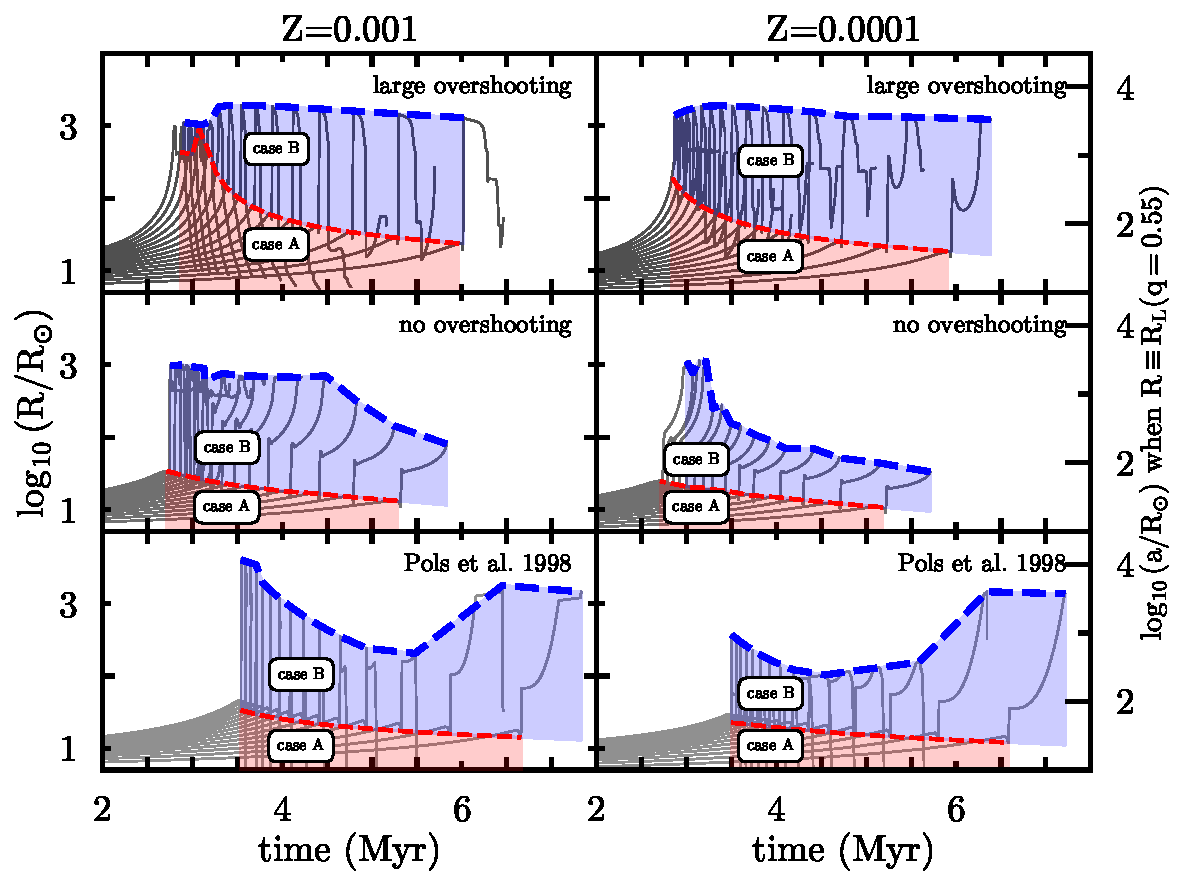
\includegraphics[width=0.9\textwidth]{radii}
  \caption{Each panel contain 15 stellar models spanning from a
    $30 \, M_{\odot}$ star on the right to a $100 \, M_{\odot}$ with
    intervals of width $5 \, M_{\odot}$. The top panels plot models
    that feature broad convective boundary mixing, the middle panels
    plot models that do not feature overshooting, and the bottom
    panels plot models generated from COMPAS using data from
    \cite{pols:98}. The left panels have a metallicity $Z=0.001$ and
    the right panels have a metallicity $Z=0.0001$}
  \label{fig:radii}
\end{figure*}


Case B is expected more often than case A mass transfer, since stars
in most mass ranges expand most prominently post-main sequence in the
Hertzsprung gap \citep{vandenheuvel:69}. However, very massive stars
may already undergo a drastic expansion in radius during their main
sequence. \citep[e.g.,][]{sanyal:15, jiang:15, sabhahit:24}. This may
increase the rate of case A \citep{demink:08}, which could have
significant implications on the rates of Wolf-Rayet+O-type binaries
\citep[e.g.,][]{nuijten:24}, X-ray binaries, and gravitational wave
progenitors. The radius of the donor is dependent on unknown stellar
parameters, including stellar winds \citep{renzo:17, josiek:24},
metallicity \citep{xin:22}, close-to-super-Eddington-layers
\citep[e.g.,][]{joss:73, paxton:13, jiang: 15, agrawal:22}, and
convective boundary mixing \citep{anders:23, johnston:24}. Here, we
illustrate this comparing the radial evolution of very massive stars
varying convective boundary mixing, metallicity, and models commonly
adopted in rapid binary population synthesis.

\section{Comparing Donor Radii}

We computed 60 MESA mode ls (version 24.03.1) from $30 \, M_{\odot}$
to $100 \, M_{\odot}$ at metallicity $Z=0.001,0.0001$ following the
setup from \cite{renzo:23} with and without overshooting and compared
them to the \cite{pols:98} models used in SSE/BSE \cite{hurley:00}
taken from COMPAS \cite{stevenson:17, vignagomez:18, riley:22}. When
using overshooting, our MESA models implement an exponential algorithm
\citep{herwig:00} fit to the step overshooting calibrated on the width
of main sequence in 30 Doradus \citep{brott:11} following
\cite{claret:18}. This relatively ``large overshooting'' model is
compared to a model that does not consider boundary mixing.

Individual models are shown in gray, and the red and blue lines in
each panel of \Figref{fig:radii} denote the maximum radius during
the main sequence and helium core burning phase respectively. The
right axis shows orbital separations where the stellar radius meets
the roche radius \citep{eggleton:83} considering a typical
accretor-to-donor mass ratio of $q=0.55$. The red regions denote
binaries which will undergo case A mass transfer and the blue regions
denote binaries which will undergo case B mass transfer. In the top
left panel, donors with masses $ \gtrsim 75 \, M_{\odot}$ can only
experience case A. Removing convective boundary mixing (middle) keeps
main sequence radii smaller, preserving the blue region at all
masses. The overshooting implementation from \cite{pols:98} (bottom),
while nonzero, still leaves a large window for case B up to
$100 \, M_{\odot}$. At even lower metallicities (right), stars are
more compact, and all models allow for case B mass transfer at all
masses.

\section{Implications for Post-Mass-Transfer Binaries}

Convective boundary mixing \cite{brott:11, johnston:24} and
metallicity have a strong effect on stellar radii, which determine
when a donor fills its Roche lobe. Case A mass transfer occurs overall
on a longer (nuclear) timescale, while case B occurs on a much shorter
(thermal) timescale \citep[but see][]{klencki:22}. Moreover, the
dynamical stability of the orbit during mass transfer is sensitive to the evolutionary phase of the stars involved
\citep[e.g.,][]{claeys:14}. Therefore, whether a given binary
experiences a common envelope depends on more than just the mass
ratio. Here, we show the depence on donor mass, metallicity, and
convective boundary mixing. Comparing rows in \Figref{fig:radii}
shows that the stellar evolution models commonly used in rapid
population synthesis are qualitatively similar to our no overshooting
models, in the sense that they allow for case B mass transfer up to
inital masses of $100 \, M_{\odot}$. Given the critial role of the
mass transfer phase in many astrophysical phenomena, the fraction of
systems experiencing case A in respect to case B may significany
impact predicted rates for post mass transfer binaries, including
Wolf-Rayet+O-type binaries, X-ray binaries, and gravitational wave
progenitors. In particular, the role of the stable mass transfer
channel \citep[e.g.,][]{marchant:21, vanson:22} for binary black hole
mergers is currently hotly debated. Our results highlight that stellar
uncertainties influence the mode of mass transfer and consequently the
outcomes.


\bibliography{./donorR.bib}
\end{document}

%%% Local Variables:
%%% mode: latex
%%% TeX-master: t
%%% End:
